\documentclass[12pt]{report}
\usepackage{times}
\usepackage{graphicx}
\begin{document}



\title{YAMS - Yet Another MIPS Simulator
\\Report 2 - Project Design and Implementation}
\author{Adam Brinley Codd
\and
Ben Cotter
\and
James Milns
\and
Qian Qiao
\and
Sridhar Sarnobat
\and
Simon West}
\maketitle



\tableofcontents
\thispagestyle{empty}



\chapter{Introduction}

As was outlined in the first report, our task is to design and implement a MIPS simulator with both a console (text-only) interface and a graphical interface.  We choose to write it as a Java application and we have divided the project into four sections.

A parser will go through the input file, checking syntax and informing the user of errors.  It will produce a kind of \emph{Abstract Syntax Tree} (AST) which will be passed on to the assembler.

An assembler will take this AST and convert the instructions to machine code and store them in our \emph{Memory Manager}.

Next, a virtual \emph{Processor} will be started which will interpret this machine code and simulate the actions, including recording input or displaying output where necessary.

The fourth major part of project is the design and implementation of the \emph{Graphical User Interface} (GUI).  In the text-only version of the program, the different parts mentioned above will be brought together by a controller class.  This will read the command line options and handle the overall flow of the program.  In the GUI version, it will be the various windows of the GUI which will bring the sections together and control program flow.

Since writing the first report we have made some changes to the design.  We were originally going to use Antlr to generate our parser however we quickly discovered that Antlr is a very complicated tool to use and since our input files are very simple lines of code with no nesting of loops or complex structures, it would be much easier to write our own parser by hand.


\chapter{Detailed Designs}

\section{Lexer and Parser}

The Lexer and Parser (referred to simply as Parser in the rest of this document) has the task of reading the input assembler source file and producing an AST in the form of an instance of a {\tt LineList} class.  This class is described in figure \ref{figLineList}.

\begin{figure}[htbp]
\begin{center}
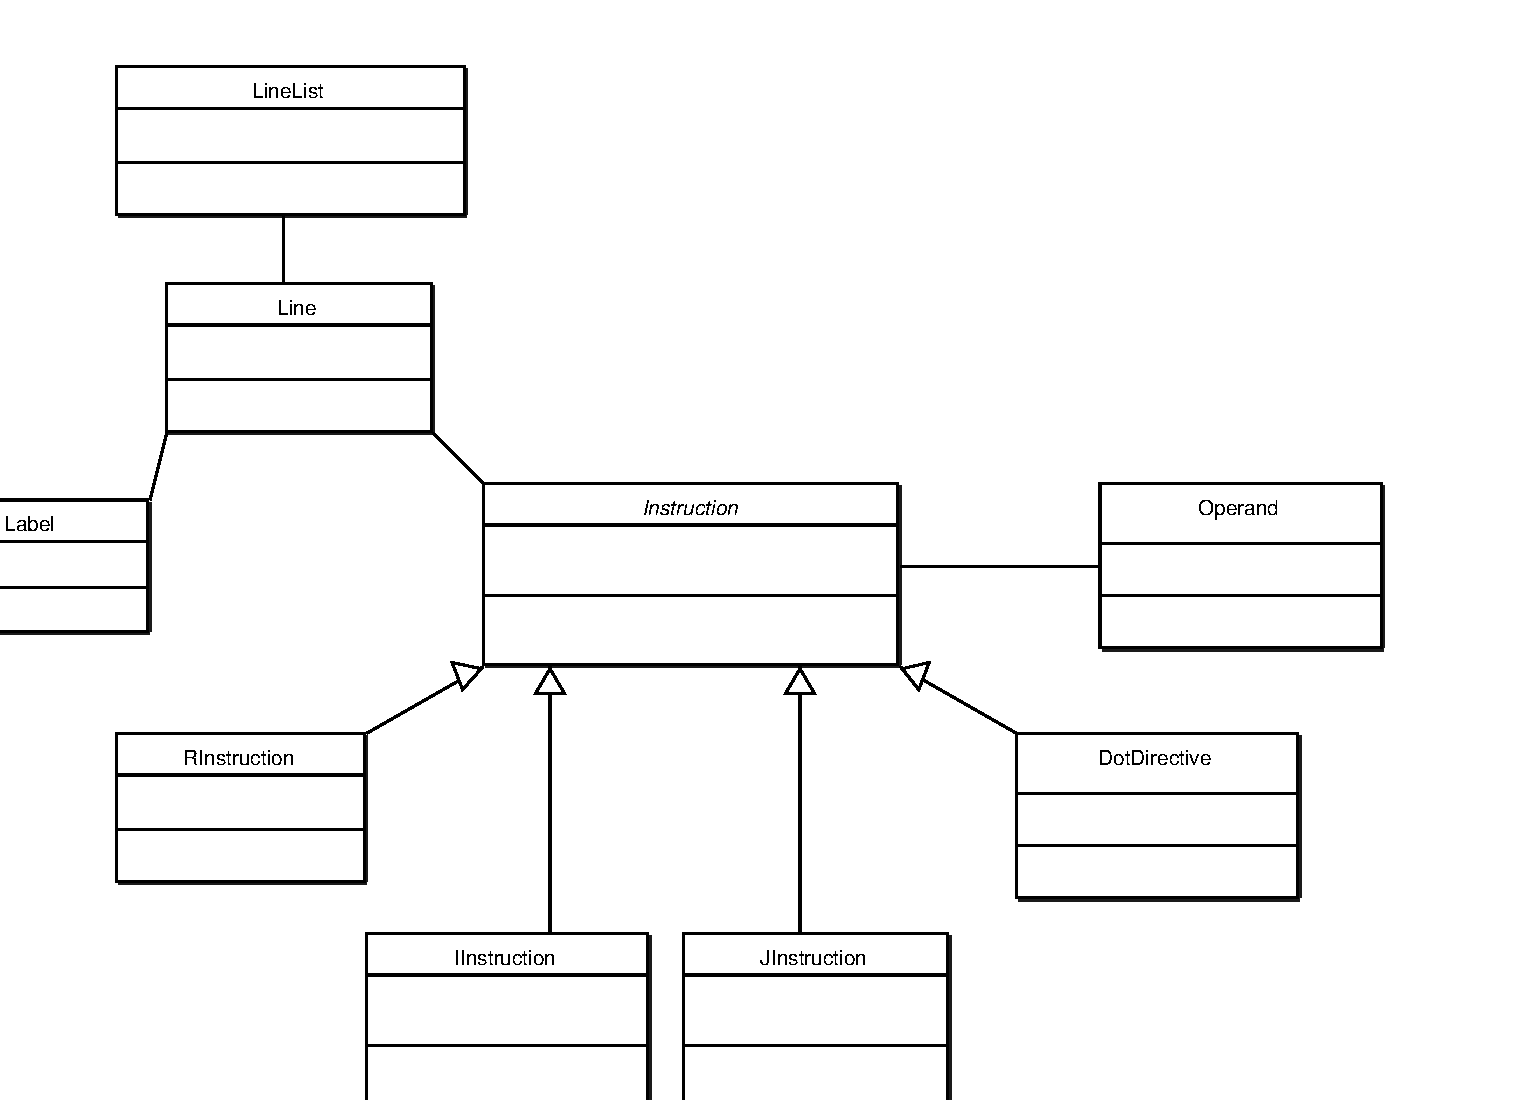
\includegraphics[height=7cm]{linelist.eps}
\end{center}
\caption{LineList}
\label{figLineList}
\end{figure}

The {\tt LineList} object contains a list of {\tt Line} objects.  Each {\tt Line} object contains either a {\tt Label}, an {\tt Instruction}, or both.  Instructions are either R-type, I-type or J-type, and depending on their type, contain either one, two or three operands.  Operands can be one of six types, as shown in figure \ref{figOperands}.

In addition, Instructions can be assembler directives, or a {\tt DotDirective} followed by any number of operands (including zero).

\begin{figure}[htbp]
\begin{center}
\includegraphics[height=7cm]{operands.eps}
\end{center}
\caption{Operands}
\label{figOperands}
\end{figure}

The Lexer takes in a string containing the text from the input file and splits it a stream of Tokens which is read by the Parser.  The parser then goes through this stream until the end of file token is reached and attempts to convert each line into an Instruction.  Any errors found at this stage are reported to the user as the process cannot continue if the Parsing isn't successful.


\section{Assembler and Loader}

When the Assembler object is created, the first thing is does is create an AssemblerXMLHandler which is used to access the XML file.  Specifically it is used to build a InstructionTable, a lookup table for instructions and their machine code representation.

The assembler takes the LineList object created by the Parser and goes through it one line at a time.

If the line contains a label, a reference is stored in the SymbolTable.

If the line contains an instruction, this is assembled to machine code using the template given {\tt InstructionTable}.  If one of the operands of the instruction contains a label, this is looked up in the {\tt SymbolTable}.  Sometimes however, a label may be encountered before it has been defined. In this case, the assembler adds a note in the {\tt ToBeDoneList} and moves on. Once it has gone through the whole {\tt LineList}, all labels should have been resolved and it can sort out the items placed in the {\tt ToBeDoneList}.

The structure of the Assembler is shown in figure \ref{figAssembler}.

\begin{figure}[htbp]
\begin{center}
\includegraphics[width=10cm]{assembler.eps}
\end{center}
\caption{Assembler}
\label{figAssembler}
\end{figure}


\section{Processor}

The {\tt Processor} is described in figure \ref{figProcessor}. Each element will be described here in detail.


\begin{figure}[htbp]
\begin{center}
\includegraphics[width=10cm]{processor.eps}
\end{center}
\caption{Processor}
\label{figProcessor}
\end{figure}

The {\tt Processor} simply acts to create and bring all the components together.  The controller, either the console program or the GUI, creates it.  It in turn creates all the other objects, the Cycle Manager, Register Manager, Memory Manager, System Call Handler, Instruction Handler, Instruction Decoder and ALU.  Interfaces for some of these objects are given in Appendix \ref{appProcessorInterfaces}.

The Cycle Manager, whilst running, executes machine code instructions which have been stored in the Memory Manager.  It looks up the current instruction using the Program Counter register from the Register Manager, and then tries to execute it using the Instruction Decoder.

The Instruction Decoder converts the instruction to a string of 32 bits in order to make it easier to work with.  It then attempts to identify which instruction it is and calls the corresponding code from the Instruction Handler (or, if it's a system call, the System Call Handler).

The Instruction Handler and System Call Handler were automatically generated from the XML file, so that the instruction set can be enlarged without changing any of the source code files.  The XML file includes a small amount of Java code for each instruction describing what it does and, of course, it has access to the Register Manager, Memory Manager and ALU.

The Register Manager and Memory Manager provide access to the Registers and Memory respectively.  In order to make the simulation as real as possible, the Memory Manager only has two public methods, {\tt getLocation} and {\tt setLocation}, which read from, and write to memory.  Similarly the Register Manager can only read and write registers.  We could have included methods to read specific bytes or bits from memory or the registers but we felt this was giving too much responsibility to what is a very simple part of the processor.


\chapter{Integration of Components and Current Status of Development}

These three parts are brought together by an overall controller class.  In the case of the console driven version, it is a simple loop which goes through the files and puts them through the Parser/Assembler/Processor, either outputting statistics or actual program output.

In the case of the GUI, it does essentially the same thing, except the operation becomes event driven rather than as a linear list of what needs to happen.  One major consequence of this is that the user can now pause the processor and step through the execution one cycle at a time.  Also, the user is able to see a graphical representation of the memory and the values stored in the registers.  Work is due to begin on this section shortly.

At the time of writing, the Parser and Processor are almost complete.  To begin with, we have been hard coding in the parts which are due to be automatically generated from XML.  These are the Instruction and System Call handlers, and parts of the Parser and Assembler.

A skeleton console controller has been written and we hope to be able to test, and demonstrate to our supervisor, the whole thing working with one simple instruction.  This will be a major step in the development process because once the XML generation is working, it will be very easy to add the rest of the instruction set.

We hope to finish these core sections by the end of next week and to have started work on the graphical user interface.


\appendix
\chapter{Processor Interfaces}
\label{appProcessorInterfaces}


\begin{verbatim}
public interface CycleManagerInterface {
  public void start();
  public void stop();
  public void terminate();
  public void advance();
  public void skip();
  public void jump(int address);
}

public interface InstructionDecoderInterface {
  public boolean handle(int instruction);
}

public interface MemoryManagerInterface {
  public void setLocation(int addr, int val);
  public int getLocation(int addr);
}

public interface RegisterManagerInterface {
  public void setReg(int regid, int val);
  public int getReg(int regid);
}
\end{verbatim}

\end{document}

